\chapter{Búsqueda de SUSY con producción electrodébil en estados finales con fotones, bosones $Z$ y Higgs}\label{cap:analysis_EWK}
% \addcontentsline{toc}{chapter}{Búsqueda de SUSY con producción electrodébil}
\chaptermark{Búsqueda de SUSY con producción electrodébil en estados finales con fotones, bosones $Z$ y Higgs}

Las búsquedas de supersimetría están caracterizadas por distintas propiedad, en particular en la que se centra esta tesis está caracterizada por la producción fuerte de gluinos, y los resultados de la misma fueron mostrados en los capítulos anteriores. De forma análoga es posible realizar una búsqueda con el mismo estado final, motivada por un modelo supersimétrico similar al anterior pero dedicado a la producción electrodébil de partículas SUSY.

La metodología empleada para realizar dicha búsqueda es similar a la búsqueda con producción fuerte, que consiste en el modelado de muestras de señal y fondo, diseño de regiones sensibles a dicho modelo, para una posterior comparación con los eventos observados. El siguiente capítulo describe los pasos seguidos hasta la realización del ajuste de solo fondo.


\section{Muestras de señal a partir de simulaciones de Monte Carlo}

El modelo que motiva a esta parte de la búsqueda es similar al descripto en la Sección \label{sec:signal_samples} con algunas salvedades. En el mismo se optimizaron los parámetros del modelo para obtener las masas y decaimientos deseados, en los cuales no estaba contemplado el decaimiento a bosones $Z$. La búsqueda electrodébil emplea una estrategia simplificada para generar las muestras de señal. En principio se fijan directamente las masas y los decaimientos de todas las partículas, sin centrarse en los parámetros de la teoría que llevan a tales valores. A su vez, la búsqueda se realiza de forma sensible a posibles decaimientos del \ninoone a fotones, bosones $Z$ y Higgs. La Figura \ref{fig:EWK_GGM_diagrams} muestra posibles diagramas de decaimiento para la búsqueda electrodébil.


\begin{figure}
  \centering
  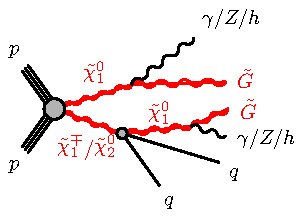
\includegraphics[width=0.45\textwidth]{images/N1N2C1-qqZhphGG-GGM.pdf}%
  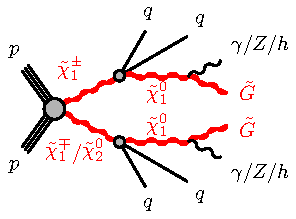
\includegraphics[width=0.45\textwidth]{images/C1C1N2-qqqqZhphGG-GGM.pdf}
  \caption{Diagramas de producción de gauginos con estado final de fotones, bosones $Z$, Higgs y gravitinos}
  \label{fig:EWK_GGM_diagrams}
\end{figure}


Se generaron 12 puntos de señal en función de la masa del \ninoone, la cual podía tomar los valores: $150\ \gev$, $250\ \gev$, $350\ \gev$, $450\ \gev$, $650\ \gev$, $750\ \gev$, $850\ \gev$, $950\ \gev$, $1050\ \gev$, $1250 \gev$ y $1450 \gev$. Los decaimientos del mismos se fijaron a $33\%$ de igual forma para $\gamma + \gravino$, $Z + \gravino$ y $h + \gravino$. Los estados finales de cada evento están caracterizados por los posibles decaimientos de los dos \ninoone de la cadena de decaimiento, los cuales pueden ser $\gamma\gamma$, $\gamma Z$, $\gamma h$, $ZZ$, $Zh$ y $hh$ (omitiendo los \gravino por simplicidad). Al estar permitidos todos los decaimientos es posible realizar un ponderado de los eventos, con el objetivo generar todas las combinaciones de decaimiento posibles. Es decir, que aquellos decaimientos que no sean de interés se les asigna un peso menor con respecto a los que se desea estudiar. Esto permite analizar múltiples modelos utilizando una sola muestra, y además calcular posibles límites de exclusión en función de las fracciones de decaimiento.

Cada modelo está caracterizado por un conjunto de fracciones de decaimientos que genera un par de partículas en el estado final. A nivel generador de las muestras es posible saber cuáles partículas se generaron y aplicarles un peso al evento dependiendo de eso. El peso que se aplica a cada evento, dependiendo del par de partículas producido y en función de las fracciones de decaimientos es:


% \begin{equation}
% \begin{split}
%   \textbf{w}(\text{BR}_{\gam}, \text{BR}_{Z}, \text{BR}_{h^{0}})  = &\ [w_{\gam\gam}, w_{\gam Z}, w_{\gam h^{0}}, w_{ZZ}, w_{Zh^{0}}, w_{h^{0}h^{0}}] \\
%      = &\ \left(\frac{1}{3}\right)^{-2} \cdot [\text{BR}_{\gam}^{2}, \text{BR}_{\gam}\cdot\text{BR}_{Z}, \text{BR}_{\gam}\cdot\text{BR}_{h^{0}}, \text{BR}_{Z}^{2}, \text{BR}_{Z}\cdot\text{BR}_{h^{0}}, \text{BR}_{h^{0}}^{2}] \\
% \end{split}
% \end{equation}


\begin{equation}
  w(\text{BR}_{\gamma}, \text{BR}_{Z}, \text{BR}_{h^{0}})=\left(\frac{1}{3}\right)^{-2}\cdot\begin{cases}
    \text{BR}_{\gamma}^{2} & \text{si el par es } \gamma\gamma \\
    \text{BR}_{\gamma}\cdot\text{BR}_{Z} & \text{si el par es } \gamma Z \\
    \text{BR}_{\gamma}\cdot\text{BR}_{h^{0}} & \text{si el par es } \gamma h \\
    \text{BR}_{Z}^{2} & \text{si el par es } ZZ \\
    \text{BR}_{Z}\cdot\text{BR}_{h^{0}} & \text{si el par es } Zh \\
    \text{BR}_{h^{0}}^{2} & \text{si el par es } hh \\
  \end{cases}
\end{equation}

El peso está normalizado de tal forma que la suma de todas las probabilidades de decaimiento de la unidad. En particular, y a modo de estudio preliminar, la búsqueda se centró en dos modelos: el modelo equivalente al de producción fuerte, donde el \ninoone decaía $50\%$ a $\gamma + \gravino$ y $50\%$ a $\gamma + h$, denominado modelo `ph+h' donde $w(0.5, 0, 0.5)$. Y el modelo donde el \ninoone decaía $50\%$ a $\gamma + \gravino$ y $50\%$ a $\gamma + Z$, denominado modelo `ph+Z' donde $w(0.5, 0.5, 0)$.

Las masas del \ninotwo y \chinopm se eligieron levemente degeneradas, e iguales a la del \ninoone más $10\ \gev$ y $11\ \gev$ respectivamente. Sus decaimientos se fijaron en $100\%$ al \ninoone a través de un $Z$ o $W$ virtual, con sus respectivos decaimientos del SM. Todas las demás partículas SUSY se desacoplaron con una masa de $4500\ \gev$. A partir de ellos se consideraron todos los posibles canales de producción electrodébil, los cuales eran: $\ninoone \ninotwo$, $\ninoone \chinoonepm$, $\ninotwo \chinoonepm$ y $\chinoonep \chinoonem$. La sección eficaz de producción de cada uno se calculó utilizando \texttt{RESUMMINO-3.0.0} \cite{Beenakker:1999xh,Debove:2010kf,Fuks:2012qx,Fuks:2013vua,Fiaschi:2018hgm} con una precisión de NLO+NLL, utilizando la familia de PDFs \texttt{CTEQ6.6} y \texttt{MSTW2008}, siguiendo las recomendaciones de \texttt{PDF4LHC} \cite{Butterworth:2015oua}. La Figura \ref{fig:SUSY_EWK_xs} muestra las secciones eficaces de cada proceso junto con la total.

\begin{figure}
  \centering
  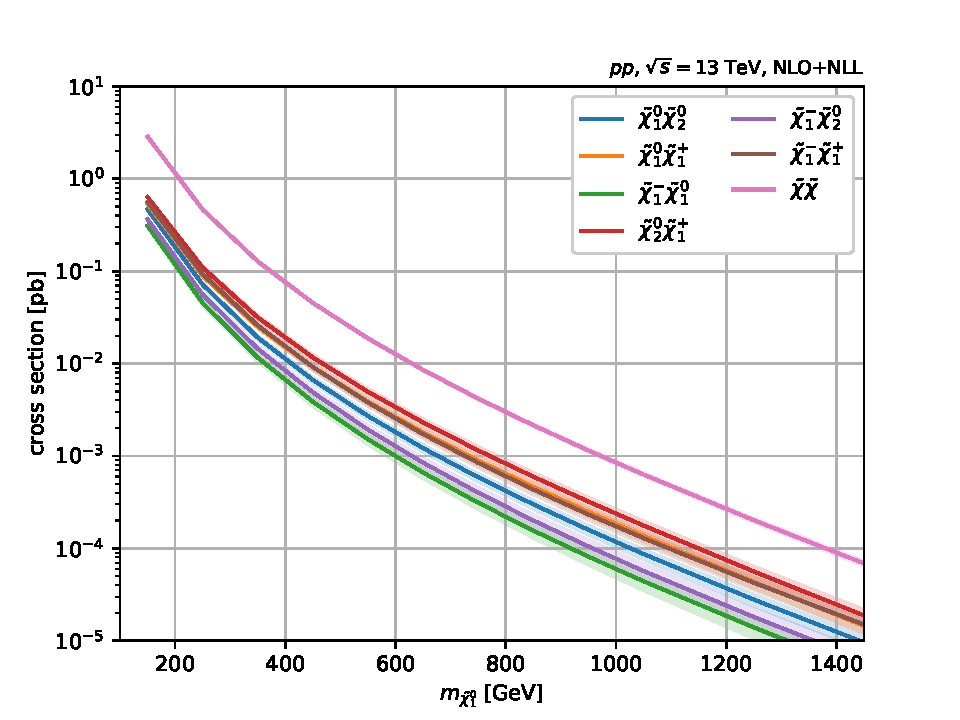
\includegraphics[width=0.7\textwidth]{images/SUSY_EWK_xsecs_m.pdf}
  \caption{Sección eficaz de la producción de gauginos en función de la masa de \ninoone. En rosa la sección eficaz total considerando todos los procesos.}
  \label{fig:SUSY_EWK_xs}
\end{figure}



\section{Fondos del Modelo Estándar}

